\label{patterns}
\subsection{Invloed van GRASP patterns}
\label{grasppatterns}
\subsubsection{Algemeen}
In onze implementatie proberen we in de meeste gevallen zo generisch mogelijk te werken. Dit heeft als indirect gevolg dat de koppeling in ons domeinmodel zeer laag is. Immers dient bij een generische implementatie abstractie gemaakt te worden van de details in de ongekende subklassen. Bijgevolg zijn enkel koppelingen zoals deze tussen \texttt{Emergency} en \texttt{Unit}, of naar de klassen van hun attributen van belang.
\subsubsection{Polymorphism}
Het pattern \textit{Polymorphism} dient vervolgens de ontbrekende details in te vullen. E\'en concreet voorbeeld hiervan is de \texttt{Emergency.calculateUnitsNeeded()} methode. Hierbij dient een specifiek type \texttt{Emergency} zelf uit te maken welke en hoeveel units er naar deze \texttt{Emergency} gestuurd moeten worden, en wat de beleidsregels zijn. Dit beantwoordt bovendien ook aan het \textit{Information Expert} patroon. Een Emergency zelf weet immers het best hoe er gereageerd dient te worden.
\paragraph{}
Ook hebben we zoveel mogelijk attributen proberen te groeperen in enumeraties. Zo hebben we bijvoorbeeld een \texttt{EmergencyStatus}, \texttt{EmergencySeverity} en \texttt{FireSize}. Dit heeft tot gevolg dat indien er bijvoorbeeld een nieuwe status toegevoegd wordt aan het model, we niets aan de \texttt{Emergency} zelf moeten veranderen. Dit is een voorbeeld van \textit{Protected Variation}. Een ander voorbeeld hiervan is onze interface \texttt{TimeSensitive}. \texttt{TimeSensitive} zegt dat het object die deze interface implementeert, afhankelijk is van de tijd. Voorlopig zijn dat enkel objecten van de klasse \texttt{Unit}. Maar als in de toekomst een \texttt{Hospital} tijdsafhankelijk wordt, dan kan dit ziekenhuis eenvoudig deze interface implementeren. Analoog werkt dit uiteraard ook voor bijvoorbeeld \texttt{Emergency}.
\paragraph{}
Een voorbeeld van \textit{Pure Fabrication} is de klasse \texttt{UnitsNeeded}. Deze klasse is verantwoordelijk voor de boekhouding van de toegewezen eenheden. De \textit{Cohesion} daalt immers wanneer de units verantwoordelijk zijn voor hun toewijziging aan de \texttt{Emergency}, of indien de \texttt{Emergency} zelf zijn units moet kiezen. Daarom hebben we ervoor gekozen een aparte klasse aan te maken die deze verantwoordelijkheid draagt. \texttt{UnitsNeeded} zorgt er ook voor dat er geen directe koppeling is tussen \texttt{Emergency} en \texttt{Unit}. Dit moet feitelijk ook niet aangezien een emergency bepaalde types units vereist en niet een unit zelf.
\paragraph{} Een voorbeeld van het \textit{Protected Variation} patroon is de klasse \texttt{Emergency\-Evaluation\-Criterium} en haar kind \texttt{StatusEqualityEmergencyEvaluationCriterium}. Dit zijn klassen die een zoekoperatie kunnen uitvoeren op een \texttt{EmergencyList}. Aangezien er feitelijk op elke mogelijke combinatie van de attributen van emergency een zoekoperatie bestaat hebben we een algemene klasse \texttt{EmergencyEvaluationCriterium} ge\"implementeerd. Deze stelt gewoon een zoekoperatie voor. De zoekoperatie zelf wordt dan gespecifieerd in een kind van deze klasse.
\paragraph{}
Voorbeelden van het \textit{Controller} patroon zijn er ook genoeg. Namelijk heel de package \texttt{projectswop201-}\\\texttt{02011.controllers}. Deze dienen als koppeling tussen de user interface en het feitelijke systeem. Aangezien een controller maar heel weinig functionaliteit mag bezitten, zijn deze klassen dan ook bijzonder kort.
\paragraph{}
Ook hebben we systematisch een lijst-klasse gemaakt wanneer er een klasse verbonden moet worden met \texttt{World}. Zo hebben we \texttt{EmergencyList}, \texttt{MapItemList} en \texttt{TimeSensitiveList}. Zoals de namen al doen vermoeden, groeperen deze lijsten objecten van een gelijknamige klasse. Zo bevat \texttt{EmergencyList} een lijst van emergencies, \texttt{MapItemList} een lijst van \texttt{MapItem}s enzovoort. Hierdoor heeft de klasse \texttt{World} een minimaal aantal verantwoordelijkheden. Zo is het niet de bedoeling dat \texttt{World} een sortering moet uitvoeren op zijn emergencies. Tevens is dit ook niet de verantwoordelijkheid van een emergency zelf. Een elegante oplossing is een nieuwe klasse tussen \texttt{World} en \texttt{Emergency} toevoegen. Deze klasse heeft dan als verantwoordelijkheid de emergencies op te slaan en eventueel operaties op deze lijst uit te voeren. Het is niet de bedoeling dat \texttt{EmergencyList} operaties op \texttt{Emergency} zelf gaat uitvoeren. \texttt{MapItemList} en \texttt{TimeSensitiveList} hebben we analoog ge\"implementeerd. Dit is dus een voorbeeld van \textit{Pure Fabrication} met als gevolg dat de \textit{Cohesion} stijgt. Ook het \textit{Indirection} patroon is hier gedeeltelijk aan de orde.
\subsection{Invloed van Design patterns}
\label{designpatterns}
\subsubsection{Composite}
\paragraph{}
We stellen onze constraints op onze emergency voor als een boom. Deze implementatie is een toepassing van het \textit{Composite} pattern. Hierbij zien we \texttt{Dispatch\-Units\-Constraint} in de rol van \texttt{Component} en de \texttt{Number\-Dispatch\-Units\-Constraint} is \'e\'en van de eventueel later uitgebreide \texttt{Leaf}s. Tot slot zien we \texttt{And\-Dispatch\-Units\-Constraint} als de \texttt{Composite} klasse. Gegeven de specificaties in de opgave is dergelijke structuur misschien ``overkill''. We zijn echter makkelijk in staat om nieuwe types constraints toe te voegen, net als connectoren (zoals bijvoorbeeld een OR). Het uitgewerkte UML diagram met de relevante methodes staat op figuur \ref{fig:compositePattern}.
\begin{figure}[h!]
\includegraphics[width=1.0\textwidth]{CD_compositePattern.pdf}
\caption{UML diagram van de implementatie van het \textit{Composite}-pattern in het project.}
\label{fig:compositePattern}
\end{figure}
Tot slot kan opgemerkt worden dat in het boek er operaties in de Composite-participant gedefinieerd worden. In deze implementatie voegen we eenvoudigweg geen operaties toe. Het kennen van de parent levert voor \verb+AndDispatchUnitsConstraint+ geen meerwaarde op. Verder kan geargumenteerd worden dat de opbouw van de boom hiermee vastligt: bottom-up. Er kan dus bijgevolg geen boom met een tak naar zichzelf bestaan. Tot slot geeft het ook de mogelijkheid om een object op verschillende plaatsen in de boom in te voegen. Dit geeft de structuur dus meer dynamiek.
\subsubsection{State}
Hoewel we geen \verb+cancel+-emergency use case moesten implementeren, anticipeerden we toch op de creatie van nieuwe toestanden waarin een emergency zich kan bevinden. We modelleerden dan ook een toestandsdiagram zoals op figuur \ref{fig:stateDiagramEmergency}.
\begin{figure}[h!]
\centering
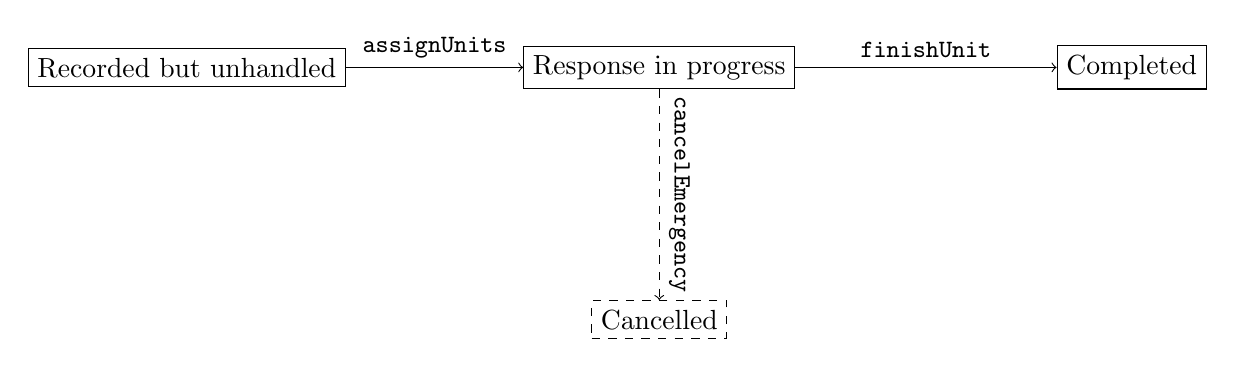
\begin{tikzpicture}
\node[rectangle,draw=black] (RBU) at (0,0) {Recorded but unhandled};
\node[rectangle,draw=black] (RIP) at (6,0) {Response in progress};
\node[rectangle,dashed,draw=black] (Cl) at (6,-3.2) {Cancelled};
\node[rectangle,draw=black] (C) at (12,0) {Completed};
\draw[->] (RBU) to node[above,midway]{\small\texttt{assignUnits}} (RIP);
\draw[->] (RIP) to node[above,midway]{\small\texttt{finishUnit}} (C);
\draw[dashed,->] (RIP) to node[above,midway,sloped]{\small\texttt{cancelEmergency}} (Cl);
\end{tikzpicture}
\caption{Beschrijving van de toestanden en overgangen van Emergency}
\label{fig:stateDiagramEmergency}
\end{figure}
Anderzijds willen we de voordelen die een \verb+enum+ ons biedt niet verliezen\footnote{Zoals bijvoorbeeld een opsomming van de verschillende toestanden.}. Daarom opteerden we voor een hybride structuur. Deze structuur behoudt in zekere zin de geest van het \textit{State}-pattern beschreven in het boek \cite{book:designpatterns}. In C++ zijn \verb+enum+s echter niet polymorf: het is een lijst van sleutels die met een binaire waarde geassocieerd worden. In Java kunnen elementen in een enumeratie in zekere zin als een singleton-subklasse van de enumeratie beschouwd worden\footnote{Uiteraard gaat die vergelijking niet volledig op.}. Het gevolg is dat we ook methodes aan deze elementen kunnen toewijzen en dus individueel anders kunnen implementeren.
\begin{figure}[h!]
\includegraphics[width=1.0\textwidth]{CD_statePattern.pdf}
\caption{UML diagram van de implementatie van het \textit{State}-pattern in het project.}
\label{fig:statePattern}
\end{figure}
Het grote nadeel van deze methode is dat alle toestanden zichtbaar zijn. Indien we dus later in het project juist een toestand willen implementeren waarover we niet kunnen filteren zal deze implementatie grondig herbekeken moeten worden. Verder biedt deze implementatie alle voordelen van het \textit{State}-pattern en een \verb+enum+.
\subsubsection{Factory Method}
Omdat units en emergencies vaak aangemaakt worden met behulp van een tekstbestand, leek het ons nuttig om hiervoor een \textit{Factory Method}-pattern te gebruiken. Op die manier kunnen we dan een set van factories bijhouden, waarbij iedere factory een bepaald directief bijhoudt. Indien bij het inlezen van het tekstbestand een directief wordt ingelezen, zal de bijbehorende factory uit de set gehaald worden, die dan vervolgens een unit of emergency aanmaakt. Hierbij werden we echter geconfronteerd met een belangrijk probleem: de parameters van de verschillende units of emergencies zijn niet uniform. We kunnen dus bijgevolg geen abstracte factorylaag bouwen waarbij de parameters gespecifieerd zijn. Dit losten we echter op door een lijst van objecten als parameter mee te geven. De implementatie is beschreven op figuur \ref{fig:factoryMethodPattern}.
\begin{figure}[h!]
\includegraphics[width=1.0\textwidth]{CD_factoryMethodPattern.pdf}
\caption{UML diagram van de implementatie van het \textit{Factory Method}-pattern in het project.}
\label{fig:factoryMethodPattern}
\end{figure}
\subsubsection{Chain of Responsibility}
Een voorbeeld van het \textit{Chain of Responsibility} pattern vinden we in de policies. Een policy is in principe een \texttt{Comparator}. Een interne methode \texttt{internalCompare} bevat de implementatie van een specifieke \texttt{Policy}. Indien deze \texttt{Policy} geen verschil kan maken tussen de twee eenheden, wordt het doorgegeven aan zijn opvolger. Deze opvolging wordt gedirigeerd door de \texttt{Compare}-methode. Pas indien er een verschil tussen twee eenheden opgemerkt wordt, of indien er geen opvolgers meer zijn, wordt het resultaat teruggegeven. Het voordeel van deze implementatie is dat ze zeer dynamisch is. Ze laat toe om het gedrag van de policy makkelijk ingrijpend te veranderen. Verder merkten we op dat de verschillende \texttt{Emergency}-implementaties meestal met dezelfde bouwstenen werkten, we besparen dus heel wat code die nodeloos gekopieerd wordt. Tot slot kunnen we ook heel eenvoudig een bouwsteen aanpassen\footnote{Wat indien bijvoorbeeld in de \texttt{ASAPPolicy} ook met een specifieke wachttijd rekening gehouden moet worden.}.
\subsubsection{Strategy}
Het \textit{Strategy} pattern vinden we terug in de policies. Elke policy is een concrete implementatie van \texttt{DispatchPolicy}. De context is hier de klasse \texttt{UnitsNeeded}. De concrete strategie\"en zijn \texttt{DefaultDispatchPolicy}, \texttt{ASAPDispatchPolicy} en \texttt{FireSizeDispatchPolicy}.
\subsection{Uitgewerkte alternatieven}
Naast dit model werden verschillende andere modellen bestudeerd. Bovendien kwam dit model ook met een zekere evolutie tot stand. Modellen werden ge\"implementeerd met een kritische blik op het ontstaan van problemen. Frequent werd dan ook het model herbekeken en aangepast. In deze sectie geven we een bondig overzicht van de belangrijkste overwogen alternatieven.
\paragraph{Domeinmodel versus klassendiagram}
Het domeinmodel in de opgave suggereert heel vaak dat bepaalde klassen dienen ge\"implementeerd te worden. Voorbeelden hierbij zijn de klassen \texttt{Caller} en \texttt{Call}. Deze werden initieel ge\"implementeerd. Er staat echter in geen enkele use case beschreven dat het bijhouden van deze instanties vereist is. Het ligt in de geest van Extreme Programming om geen functionaliteiten te schrijven die geen duidelijk nut hebben. Eenvoud ligt immers aan de basis van een goed model. Bijgevolg werd besloten deze klassen te verwijderen. Bovendien werd de implementatie zo vereenvoudigd. Iets soortgelijks gebeurde met de klassen \texttt{Operator}, \texttt{Dispatcher} en \texttt{UnitCommander}. Deze klassen zijn niet volledig verdwenen uit ons model want er bestaan nog controllers voor.
\paragraph{EmergencyDescription}
Een ander probleem is hoe we informatie over deze velden naar buiten kunnen brengen. Hiervoor construeerden we een \verb+EmergencyDescription+ klasse. Deze klasse bevat informatie over de verschillende parameters: hun type, naam en eventueel een beschrijving. Bovendien is deze beschrijving in staat om te controleren of een bepaalde lijst van objecten aan deze beschrijving voldoet.